\documentclass{article}

\usepackage{ctex}
\usepackage{tikz}
\usetikzlibrary{cd}
\usetikzlibrary{decorations.pathreplacing}

\usepackage{amsthm}
\usepackage{amsmath}
\usepackage{amssymb}

\usepackage{unicode-math}


\usepackage[textwidth=18cm]{geometry} % 设置页宽=18

\usepackage{blindtext}
\usepackage{bm}
\parindent=0pt
\setlength{\parindent}{2em} 
\usepackage{indentfirst}


\usepackage{xcolor}
\usepackage{titlesec}
\titleformat{\section}[block]{\color{blue}\Large\bfseries\filcenter}{}{1em}{}
\titleformat{\subsection}[hang]{\color{red}\Large\bfseries}{}{0em}{}
%\setcounter{secnumdepth}{1} %section 序号

\newtheorem{theorem}{Theorem}[section]
\newtheorem{lemma}[theorem]{Lemma}
\newtheorem{corollary}[theorem]{Corollary}
\newtheorem{proposition}[theorem]{Proposition}
\newtheorem{example}[theorem]{Example}
\newtheorem{definition}[theorem]{Definition}
\newtheorem{remark}[theorem]{Remark}
\newtheorem{exercise}{Exercise}[section]

\newcommand*{\xfunc}[4]{{#2}\colon{#3}{#1}{#4}}
\newcommand*{\func}[3]{\xfunc{\to}{#1}{#2}{#3}}

\newcommand\Set[2]{\{\,#1\mid#2\,\}} %集合
\newcommand\SET[2]{\Set{#1}{\text{#2}}} %

\begin{document}
\title{Mathematical Analysis}
\author{枫聆}
\maketitle
\tableofcontents

\section{极限论}
\subsection{数列极限}
数列,整序傻傻分不清....

\begin{definition}
若对于每一整数$\varepsilon$,不论它怎样小,恒有序号$N$,使在$n > N$时,一切$x_n$的指满足不等式\[|x_n-a| < \varepsilon\],则称常数$a$为整序变量$x=x_n$的极限.

$a$是整序变量的极限这一事实,记成:\[\lim x_n =a \text{ 或者 } \lim x = a\],也可以说这个序列收敛于$a$
\end{definition}

有一个很有趣的几何解释在这里,

\begin{center}
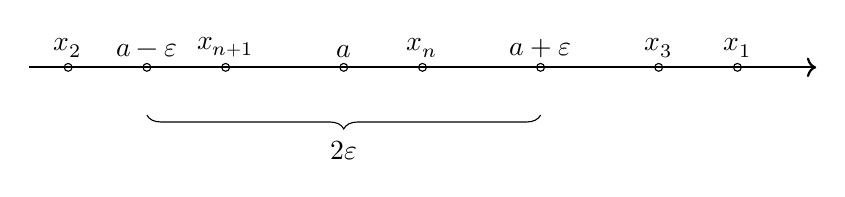
\begin{tikzpicture}
\draw[thick,->] (0,0) -- (10,0);
\draw (0.5,0) node[circle,draw,scale=0.3]{} node[above] {$x_2$};
\draw [decorate,decoration={brace,amplitude=5pt,mirror,raise=4ex}]
  (1.5,0) node[circle,draw,scale=0.3]{} node[above]{$a-\varepsilon$} -- (6.5,0) node[midway,yshift=-3em]{$2 \varepsilon$} node[circle,draw,scale=0.3]{} node[above]{$a+\varepsilon$};
%\draw [Parenthesis-Parenthesis,] (2,0) node[above] {$a-\varepsilon$} -- (7,0) node[above] {$a+\varepsilon$};
\draw (2.5,0) node[circle,draw,scale=0.3]{} node[above] {$x_{n+1}$};
\draw (4,0) node[circle,draw,scale=0.3]{} node[above] {$a$};
\draw (5,0) node[circle,draw,scale=0.3]{} node[above] {$x_n$};
%\draw (7,0) node[circle,draw,scale=0.3]{} node[above] {$a+\varepsilon$};
\draw (8,0) node[circle,draw,scale=0.3]{} node[above] {$x_3$};
\draw (9,0) node[circle,draw,scale=0.3]{} node[above] {$x_1$};
\end{tikzpicture}
\end{center}

以$a$点为中心的线段不论取的多小(其长度为$2\varepsilon$),一切$x_n$点从某点起,必全部落在这线段之内,这样在线段之外一定只有有限长度个点了,表示极限的点$a$表示整序变量的数值的点的凝聚中心.
\end{document}
